\subsection{Estrategia de acceso y actualización local}

La implementación concreta sigue el siguiente esquema operativo. Cuando una operación necesita una amplitud o un par de amplitudes, primero determina
los bloques implicados. Después consulta la caché. Si el bloque ya está disponible, reutiliza el buffer descomprimido. Si no está disponible, lo
recupera desde almacenamiento comprimido, lo inserta en la caché y continúa con la operación.

Una vez modificado un bloque, este no se recomprime inmediatamente por defecto. En lugar de ello, se mantiene en la caché marcado como sucio hasta
que sea necesario liberarlo o hasta que la operación actual requiera un vaciado explícito. Esta política evita recompresiones prematuras cuando varias
compuertas consecutivas afectan el mismo conjunto de bloques.

Para compuertas cuyas amplitudes involucradas residen en un mismo bloque, el procedimiento es completamente local. En cambio, para operaciones que
afectan amplitudes distribuidas en bloques distintos, el esquema debe adquirir ambos bloques y gestionar su permanencia en la caché. Este caso hace
evidente la necesidad de mantener al menos dos bloques activos y explica por qué la caché no puede reducirse a una sola entrada.

\begin{figure}[H]
    \centering
    \caption{Flujo de ejecución para compuertas locales sobre un único bloque}
    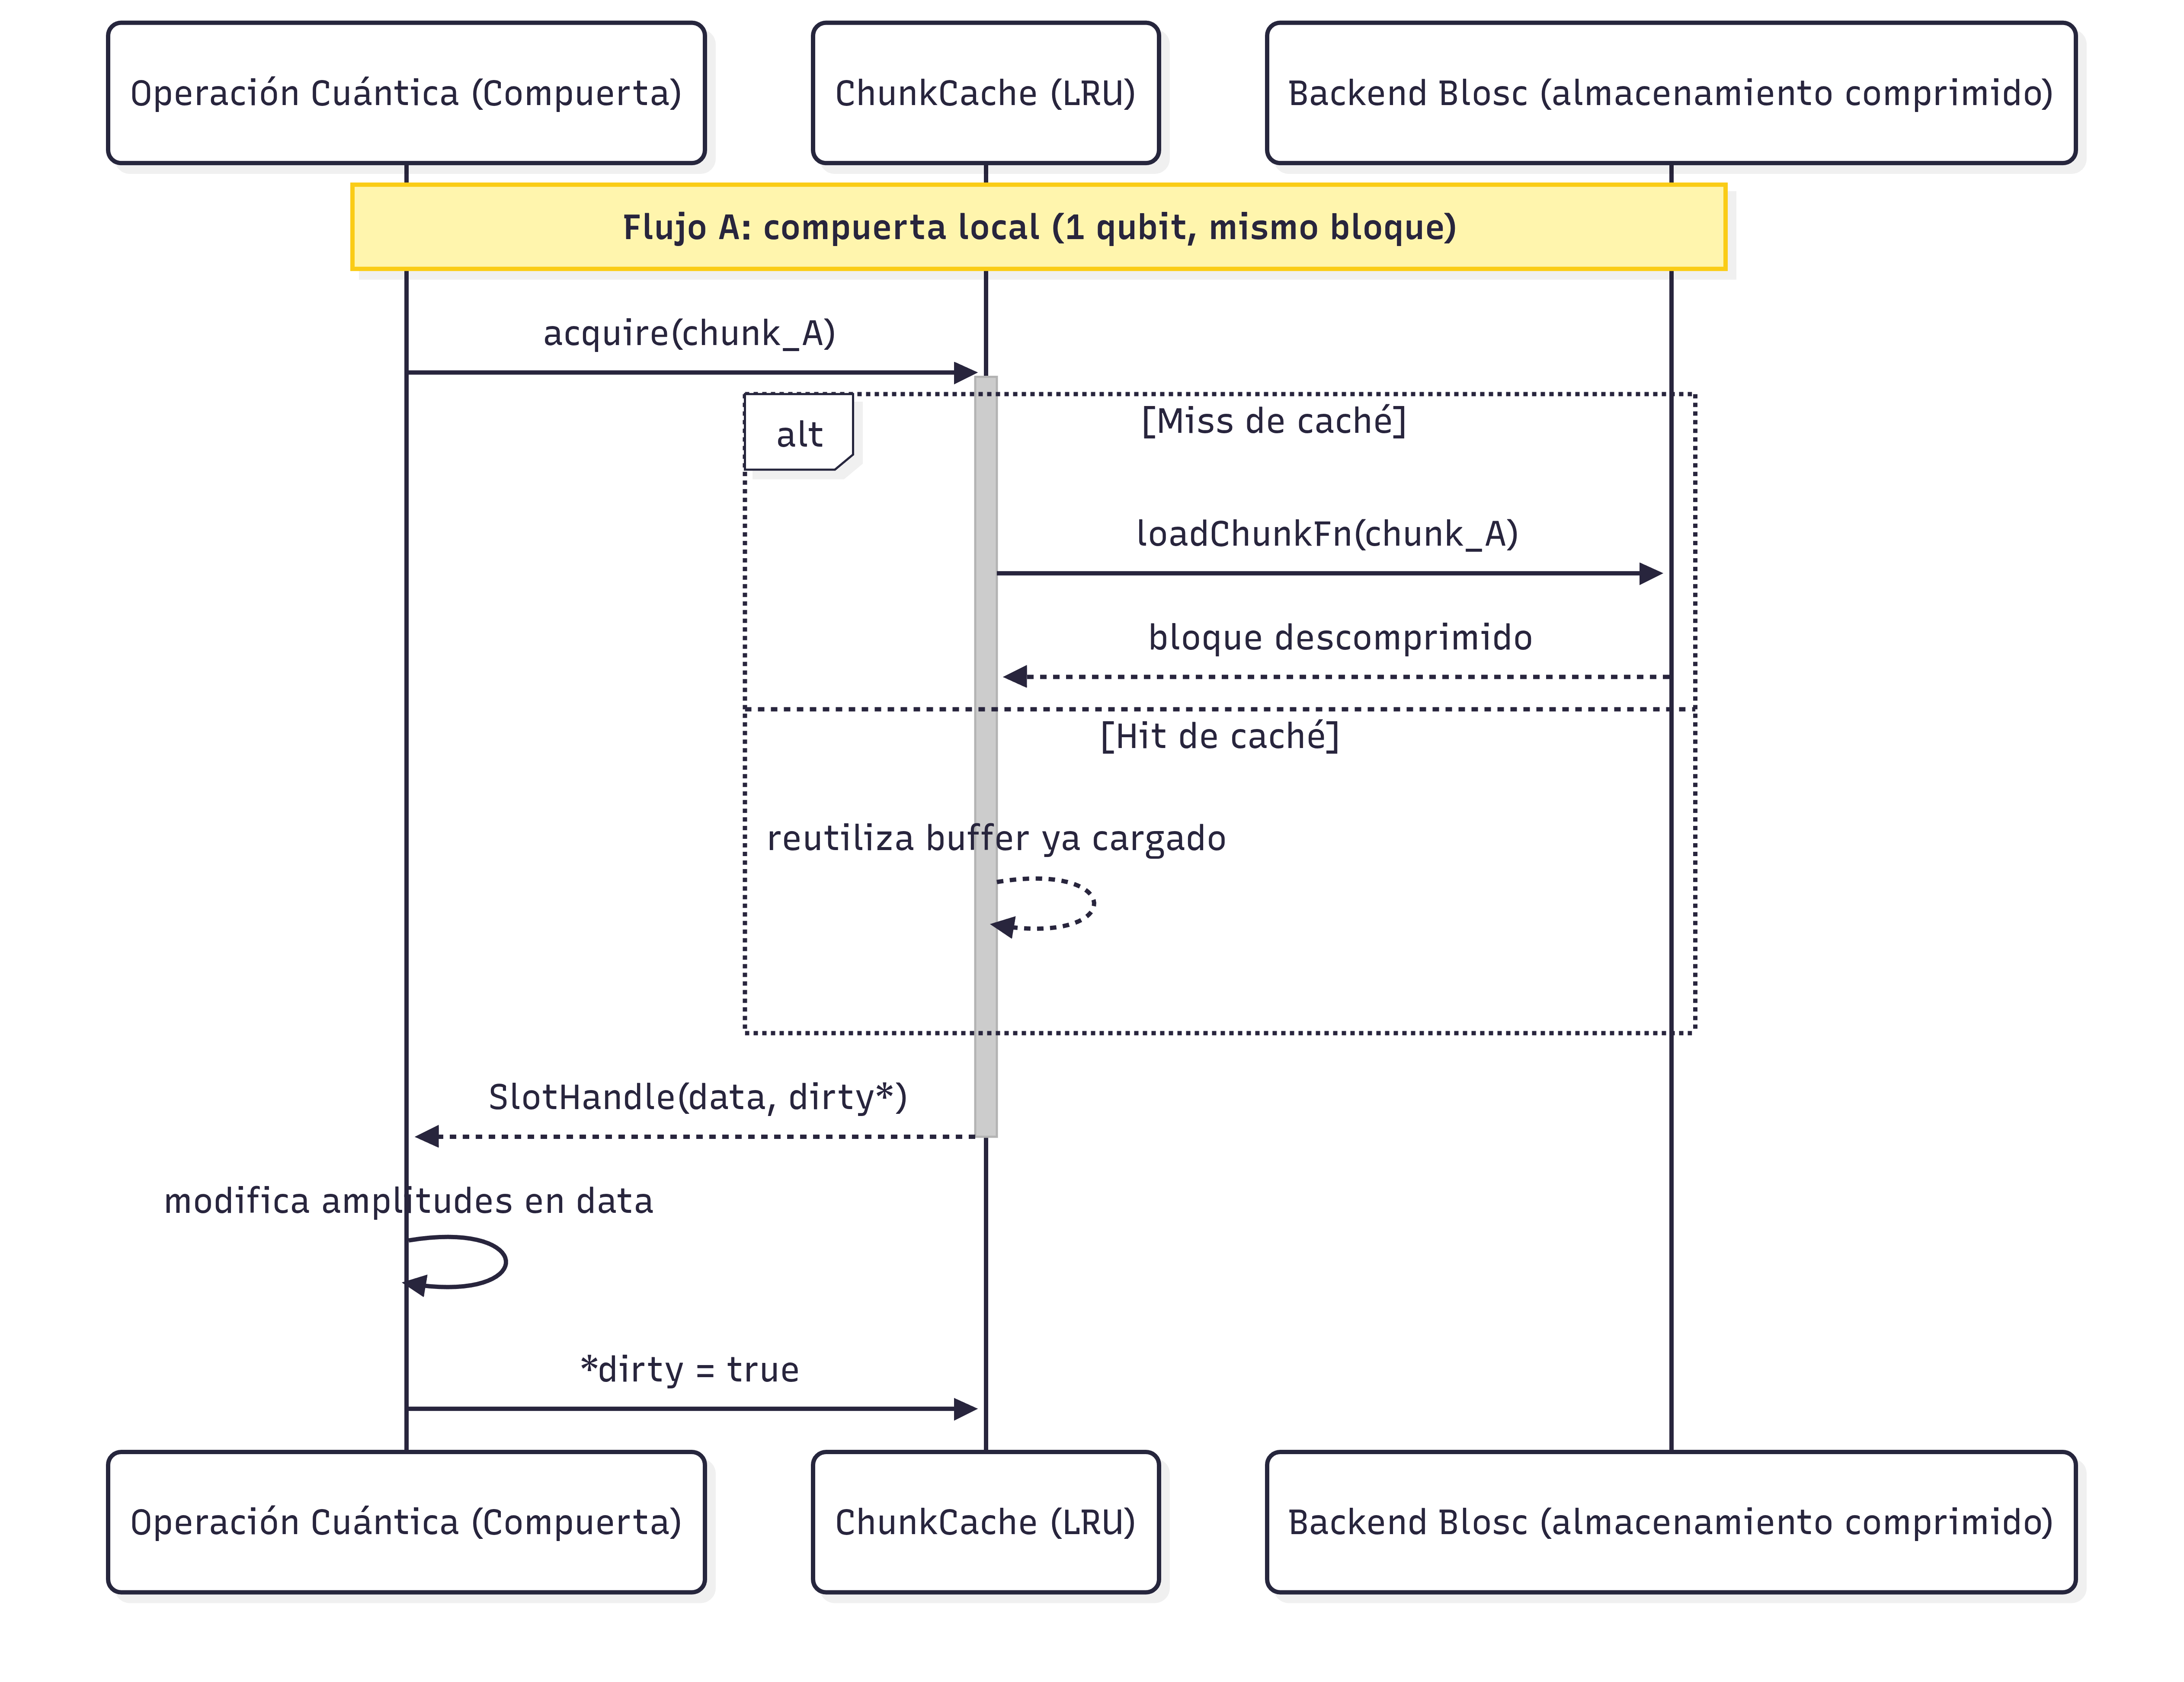
\includegraphics[width=1\textwidth]{images/development-workflow-a.png}
    \label{fig:development-workflow-a}
\end{figure}

\begin{figure}[H]
    \centering
    \caption{Flujo de ejecución para compuertas que operan entre bloques}
    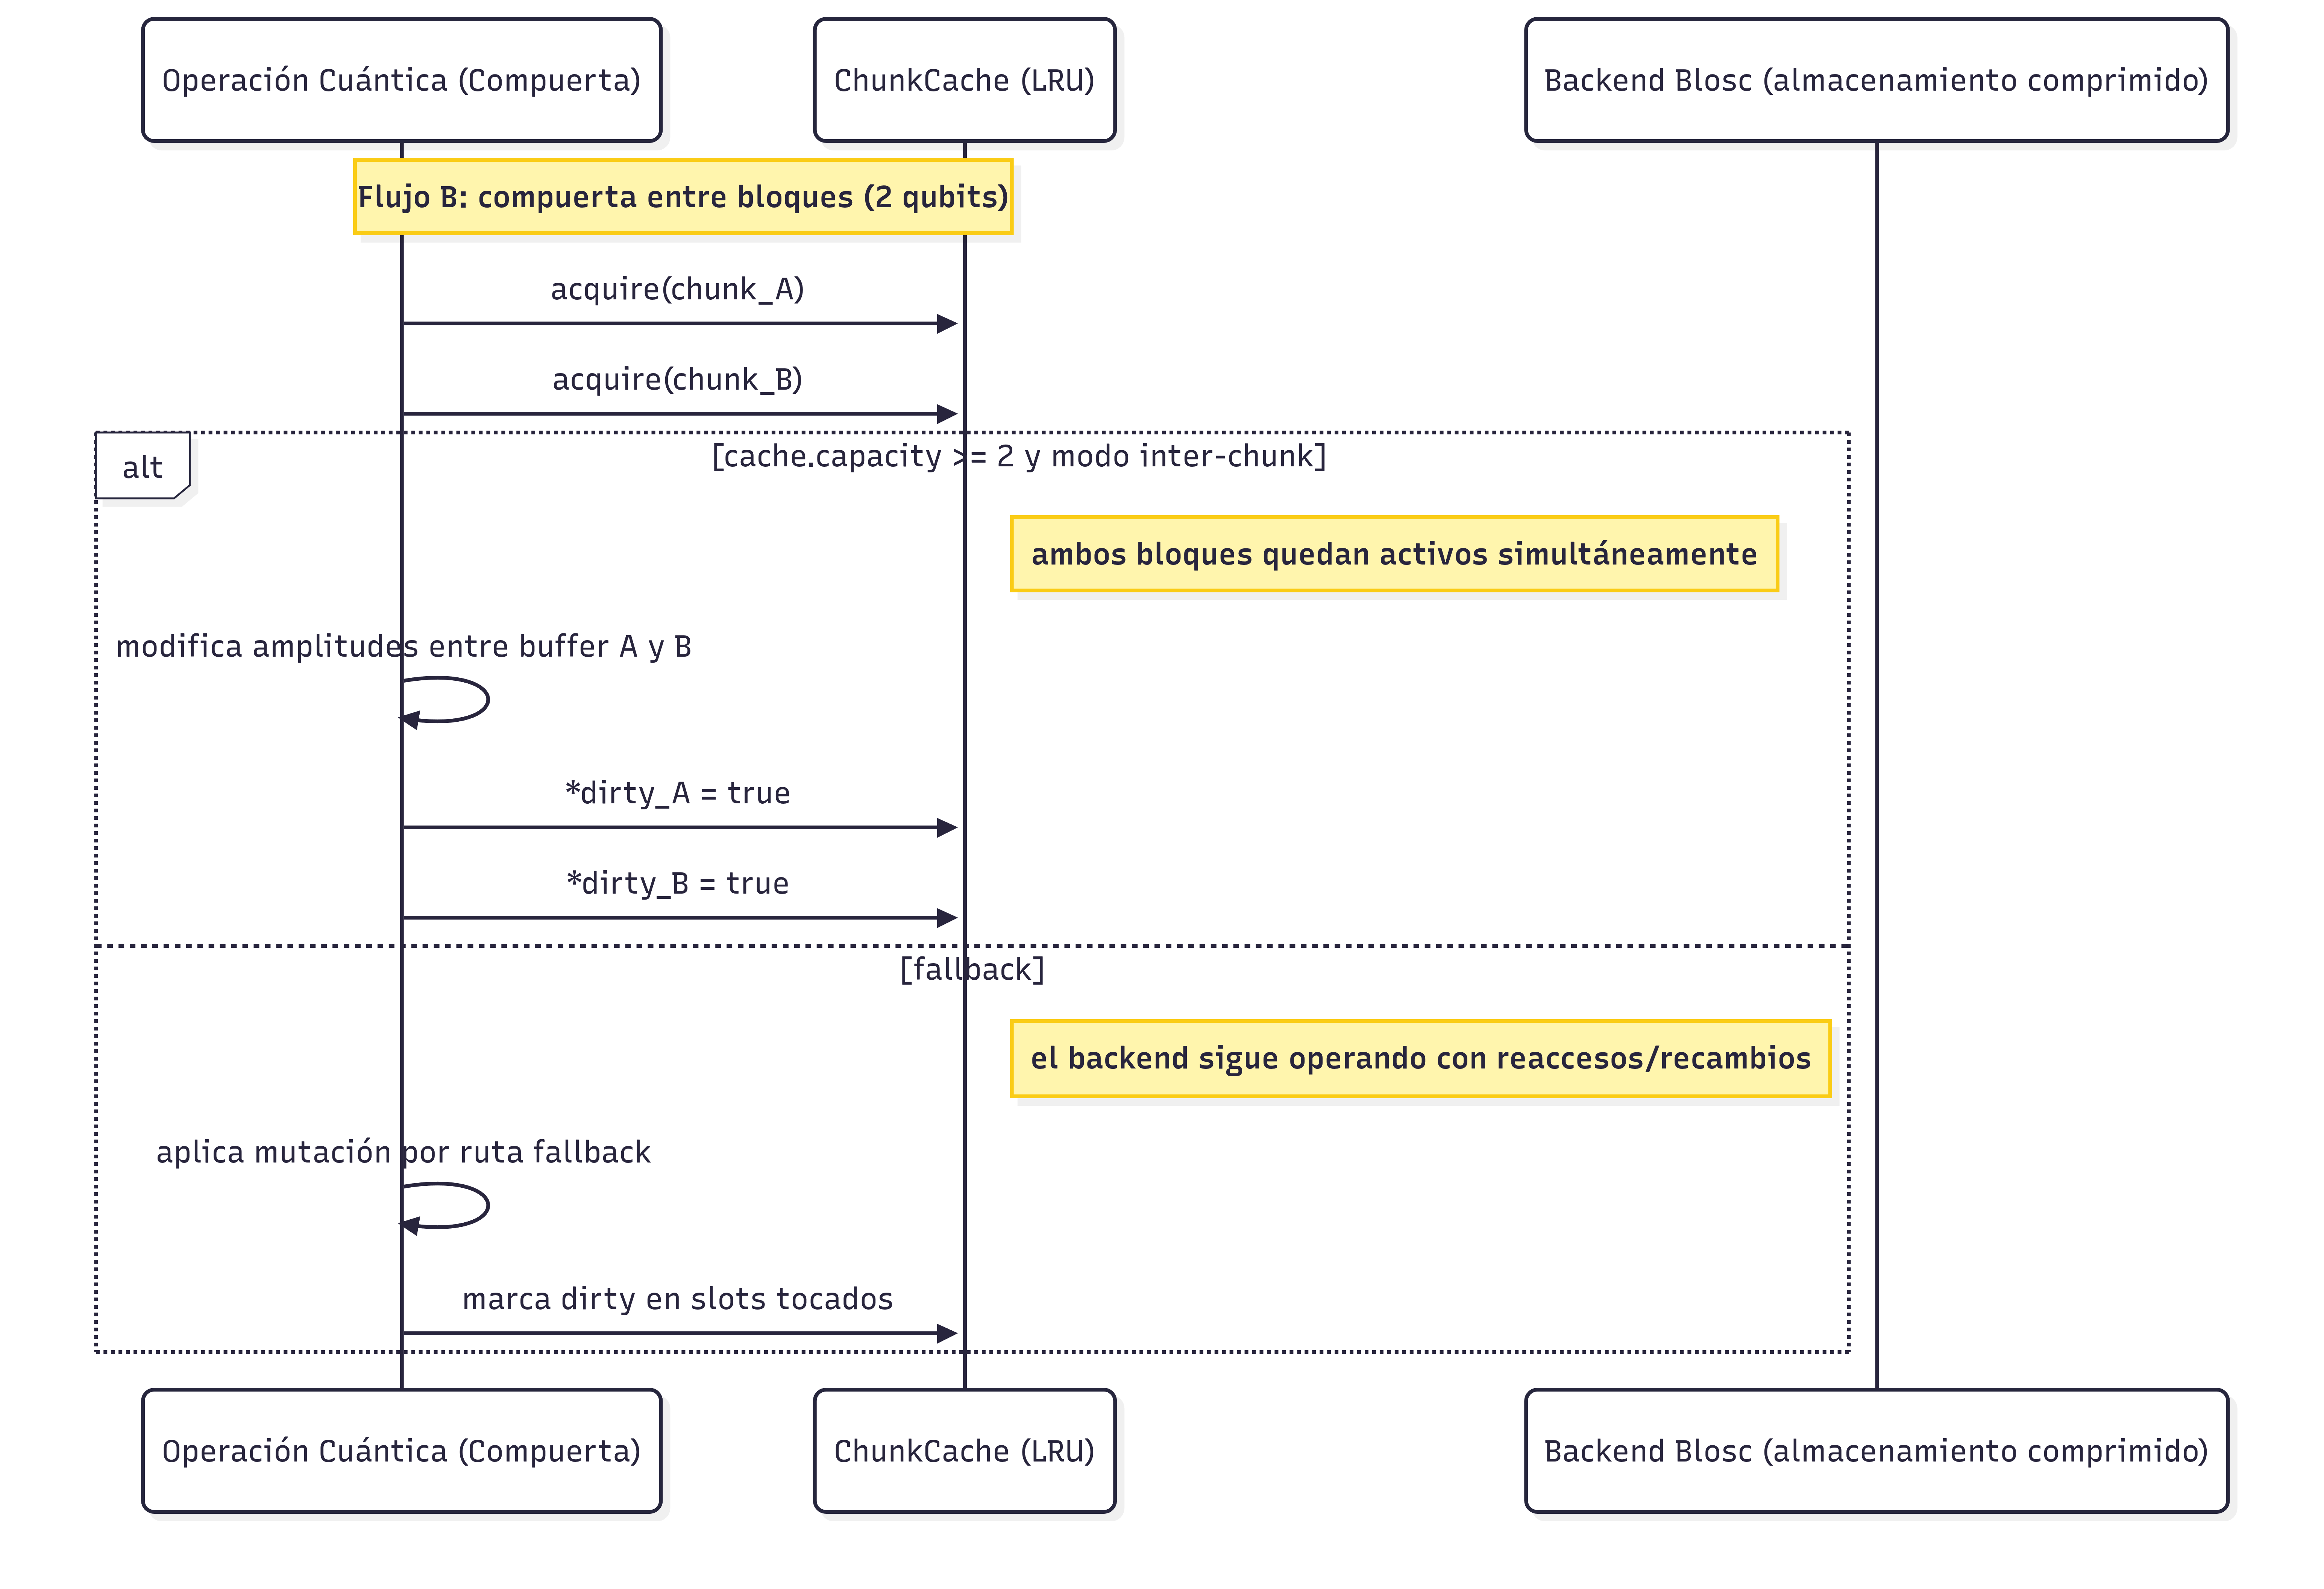
\includegraphics[width=1\textwidth]{images/development-workflow-b.png}
    \label{fig:development-workflow-b}
\end{figure}

\begin{figure}[H]
    \centering
    \caption{Flujo de persistencia diferida y escritura en backend comprimido}
    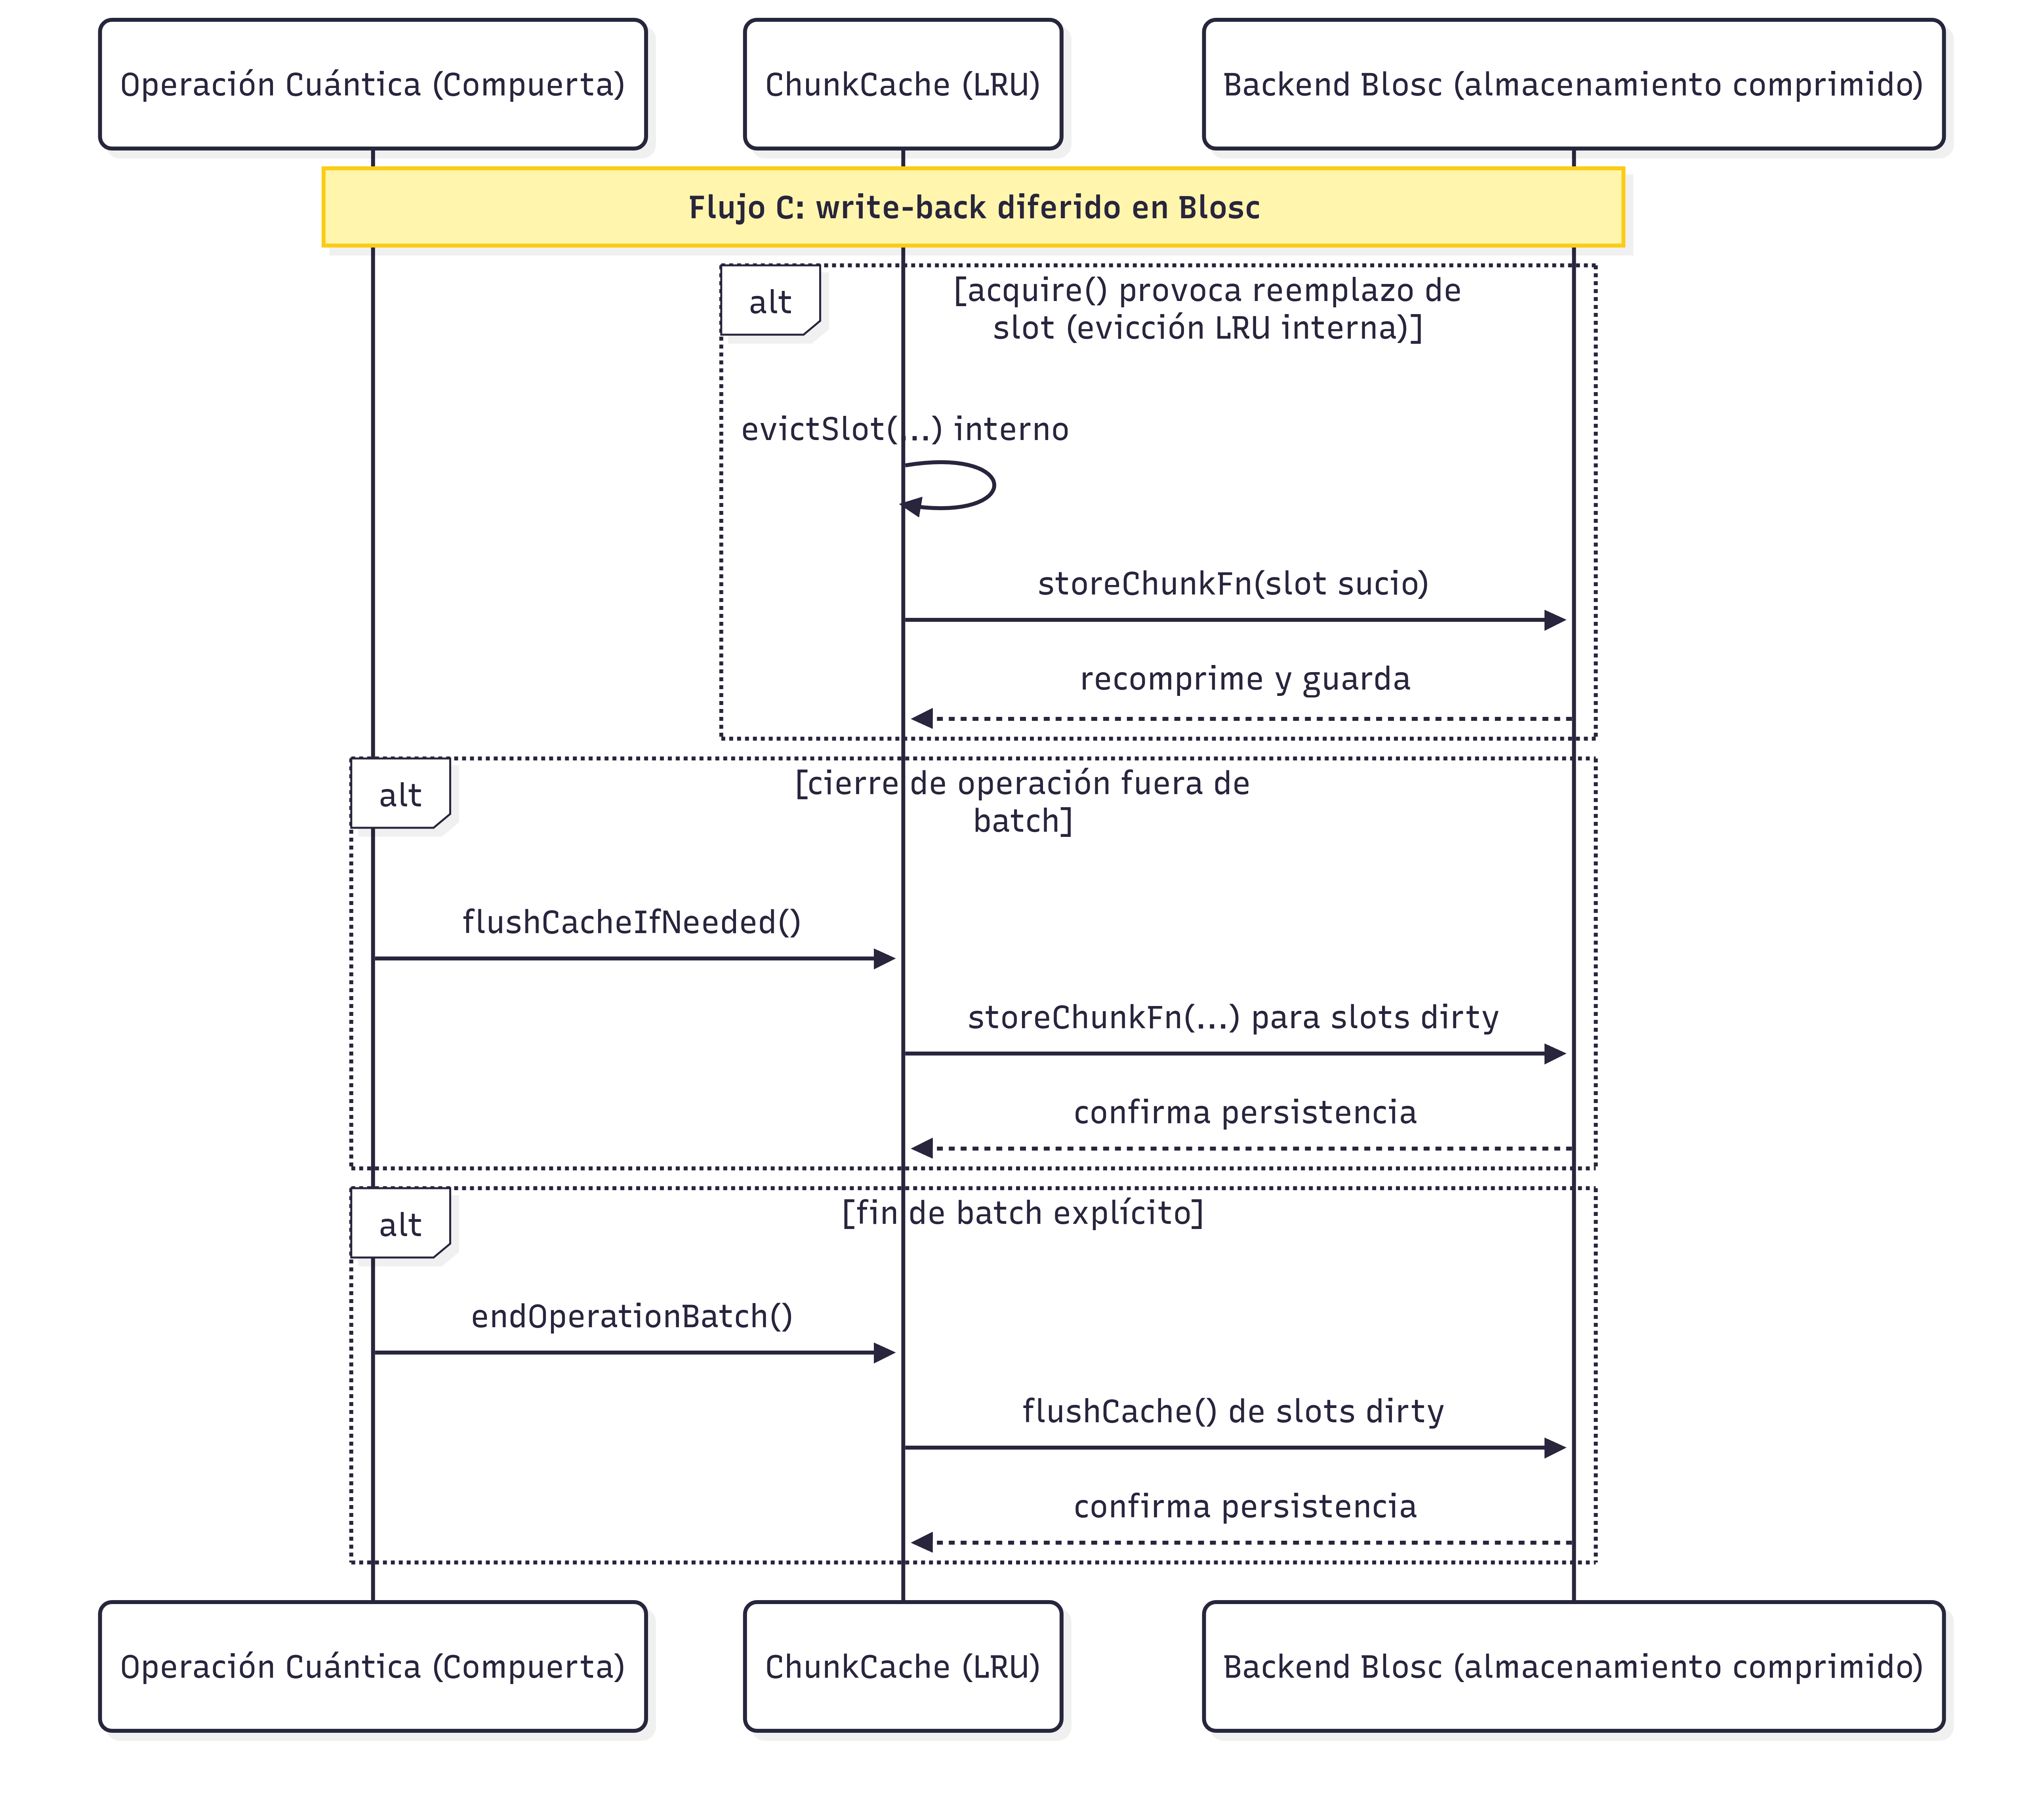
\includegraphics[width=1\textwidth]{images/development-workflow-c.png}
    \label{fig:development-workflow-c}
\end{figure}

La misma infraestructura permite exportar el vector completo de amplitudes una vez finaliza la ejecución del circuito. Esta capacidad resulta esencial para la validación del trabajo, ya que permite contrastar la representación comprimida frente a la referencia no comprimida sobre exactamente la misma instancia experimental y verificar si la igualdad de amplitudes se preserva o, en el caso con pérdida, cuantificar la discrepancia introducida.

El mecanismo descrito en este capítulo establece la base operativa para medir el efecto de la
compresión sobre circuitos representativos. La sección siguiente presenta la evaluación
experimental realizada sobre Grover y QFT, así como la comparación cuantitativa entre la
estrategia sin compresión, la estrategia sin pérdida basada en Blosc y una estrategia con
pérdida controlada basada en ZFP.
